\paragraph{Requiredfunctionality}
Our initial plans for the animation were to make it depend on the actual user input in the exercise itself, particularly taking the sequence and the primers from the previous stages of the application. This was mainly to differentiate more from other similar PCR animations, like those demonstrated to us by the clients (see Section \ref{intro:motiv}. Because of the high customisation requirements set by the task at hand and to provide maximum compatibility throughout the project we decided to develop the animation on Java utilising Java graphics package and Swing together, with the animation logic being developed from scratch. However, towards the end of the animation development it became apparent that the sequence required to be presented in the animation is just too large to be reasonably scaled with the individual bases being visible. To extrapolate, the individual bases were hard to make out as soon as the target PCR area reached about 150 bases in length, which was not enough as the area could be well over that limit. Finally, as the clients were satisfied with a static animation, it was decided that we would just use the animation with a sample input that  was adequately sized. It was also suggested by the clients that the individual base's colour coding doesn't need to be explained in the animation as it was clear enough that the different colours represent different bases. Otherwise the aforementioned shift in the overarching animation design didn't affect it in any way. The final animation sreenshots and explanation of its individual parts are provided below.

\paragraph{Implementation}
The whole animation is controlled with a large set of conditional statements by a Swing timer that constantly recalculates the time passed from the start of the animation, pausing if it reaches the end of a stage until a button press changes the stage and therefore sets the time passed to a particular value. The models used in the animation were developed in the Inkscape vector graphics editor and are the different type of the individual base's models, the Taq polymerase model and three models for three different states of the thermometer. The individual bases are then drawn to make a sequence at a particular location.

\paragraph{Functionality Explained}
The animation is split into 7 stages, each eith a related explanatory statement at the bottom. A thermometer is displayed at all times on the screen to show the current temperature at each stage of the process. Four buttons lie above the descriptive text: "Close", to close the application completely; "Restart", to go to the start of the exercise; "Previous" and "Next" to navigate between the animation stages. The animation won't proceed until the "Next" button is pressed, something which was suggested by the clients, as they pointed out that the user might not be able to read the text in the time provided. Finally, the PCR animation itself is in the top part of the screen.

\paragraph{Animation Screens}

In the stages 0 and 1, PCR is briefly explained in simple terms as the temperature rises to 72\degree C.

\begin{figure}[h]
  \begin{center}
	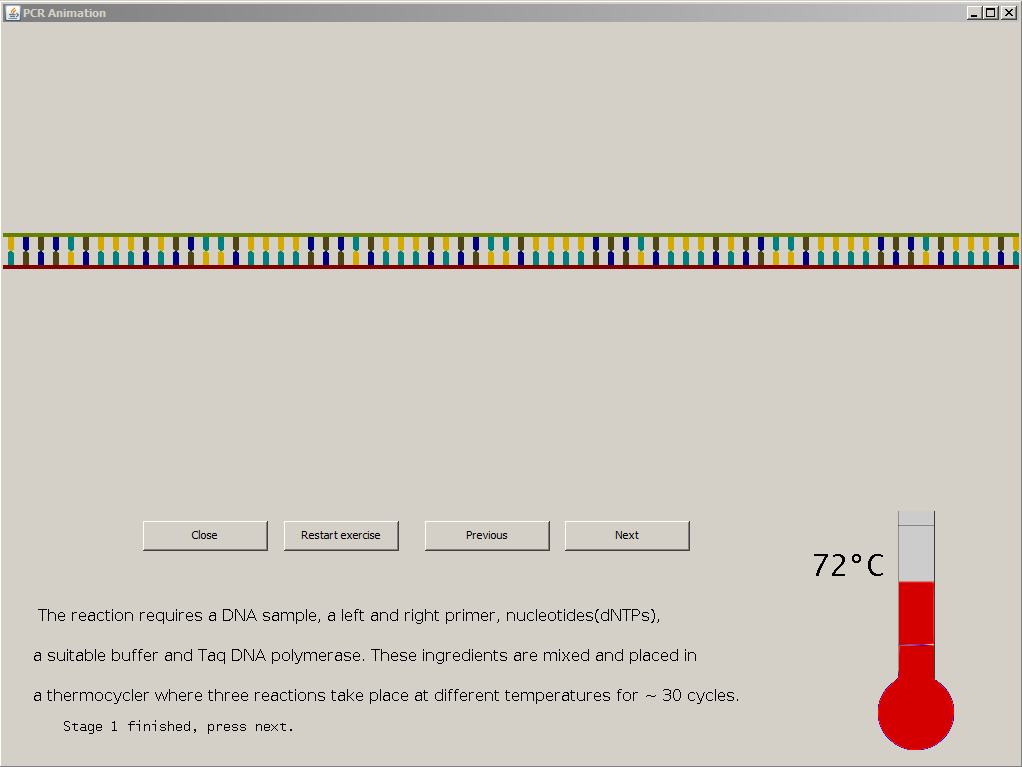
\includegraphics[width=0.6\textwidth]{./images/AnimImpl/Stage1.png}
    \caption{
      \label{fig:AnimImpl:stage1}
      Animation, Stage 1
    }
  \end{center}
\end{figure}


In stage 2, Melting and Annealing, the strands are separated and the primers bind to them, with the temperature level varying accordingly.

\begin{figure}[h]
  \begin{center}
	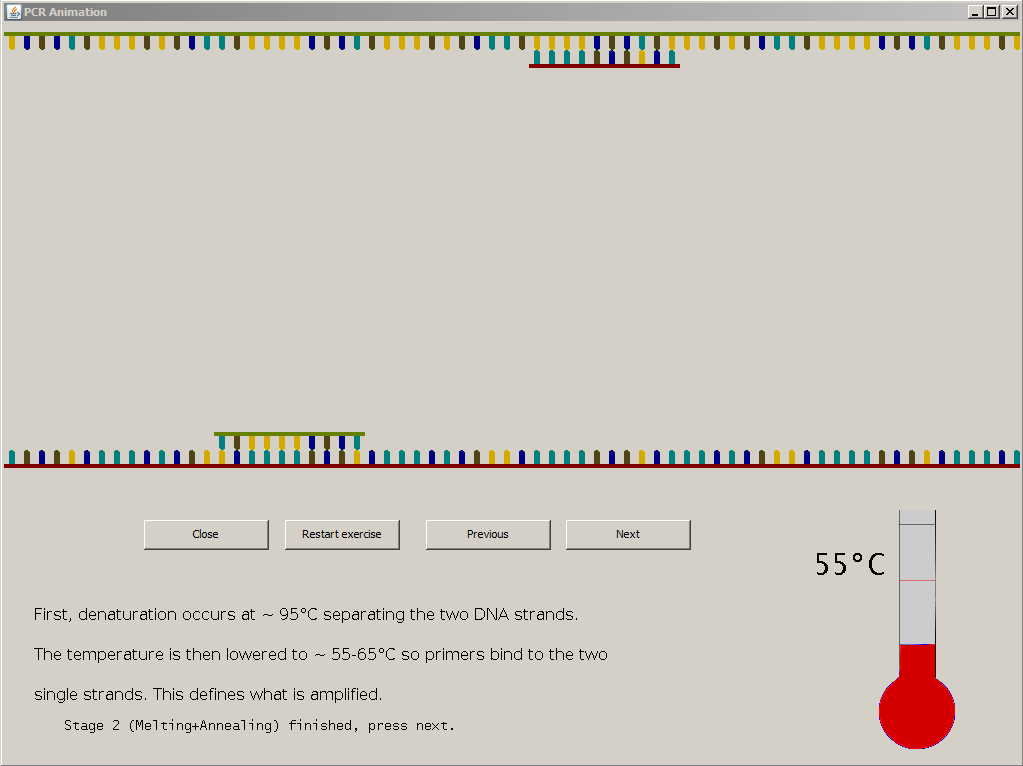
\includegraphics[width=0.6\textwidth]{./images/AnimImpl/Stage2.png}
    \caption{
      \label{fig:AnimImpl:stage2}
      Animation, Stage 2
    }
  \end{center}
\end{figure}

In stage 3, Adding nucleotides, the taq polymerase creates a complementary copy of each strand, with the temperature once again raised to 72\degree C.

\begin{figure}[h]
  \begin{center}
	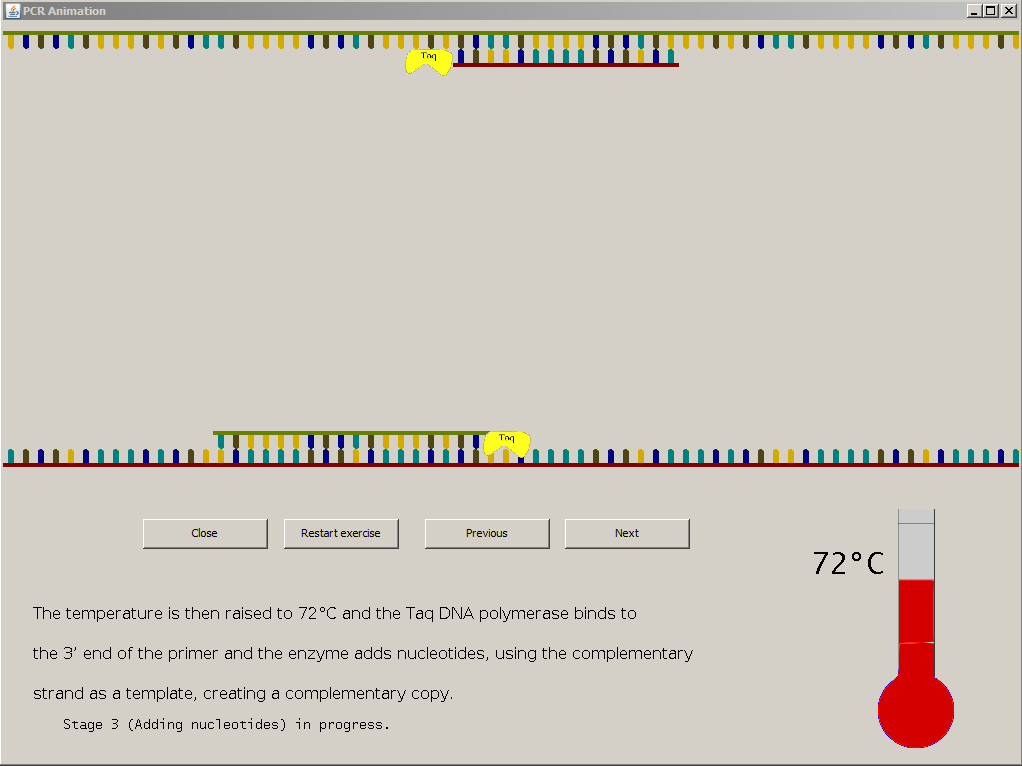
\includegraphics[width=0.6\textwidth]{./images/AnimImpl/Stage3.png}
    \caption{
      \label{fig:AnimImpl:stage3}
      Animation, Stage 3
    }
  \end{center}
\end{figure}

In stages 4 and 5 another cycle of PCR is shown and the required sequence is generated for the first time.

\begin{figure}[h]
  \begin{center}
	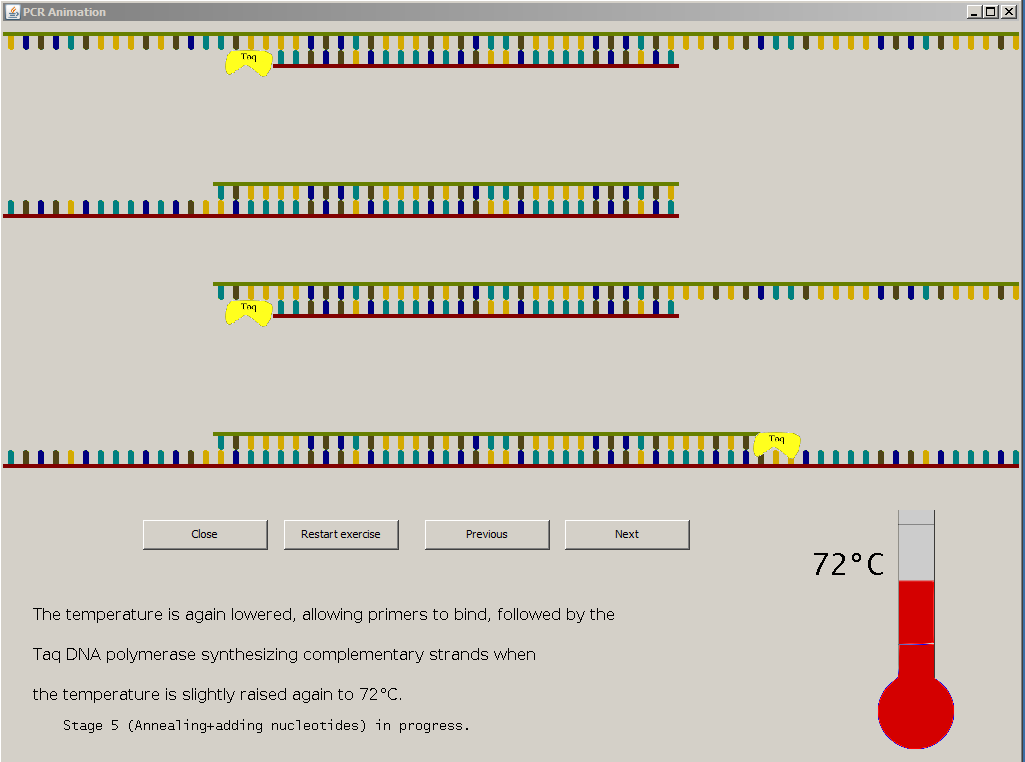
\includegraphics[width=0.6\textwidth]{./images/AnimImpl/Stage5.png}
    \caption{
      \label{fig:AnimImpl:stage5}
      Animation, Stage 5
    }
  \end{center}
\end{figure}

Finally, the last two stages explain how many copies of the target sequence is produced in subsequent cycles and the user is explained that they completed the exercise and thanked for participation.

\begin{figure}[h]
  \begin{center}
	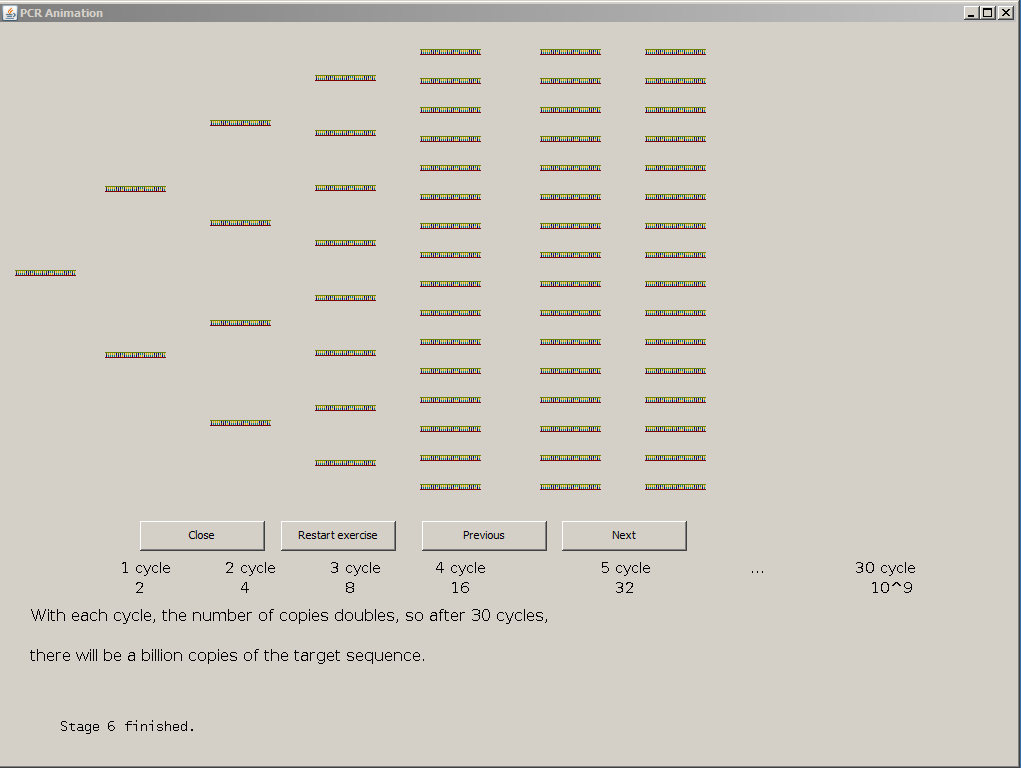
\includegraphics[width=0.6\textwidth]{./images/AnimImpl/Stage6.png}
    \caption{
      \label{fig:AnimImpl:stage6}
      Animation, Stage 6
    }
  \end{center}
\end{figure}
